
\newcommand{\nextindex}[3]{%
  % #1 = current index
  % #2 = maximum index
  % #3 = name of variable to store result
  \pgfmathtruncatemacro{\temp}{#1+1}%
  \ifnum\temp>#2
    \pgfmathtruncatemacro{#3}{1}%
  \else
    \pgfmathtruncatemacro{#3}{\temp}%
  \fi
}

\begin{figure}
\[
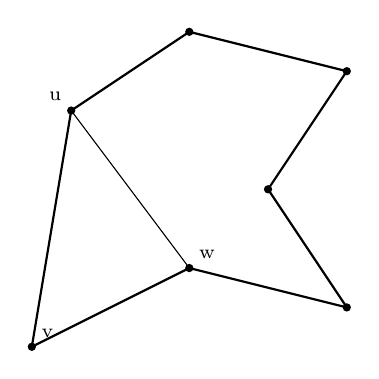
\begin{tikzpicture}[scale=1]
  \coordinate (P1) at (0,0);
  \coordinate (P2) at (2,1);
  \coordinate (P3) at (4,0.5);
  \coordinate (P4) at (3,2);
  \coordinate (P5) at (4,3.5);
  \coordinate (P6) at (2,4);
  \coordinate (P7) at (0.5,3);

  \foreach \i in {1,...,7} {
    \nextindex{\i}{7}{\next}
    \draw[thick] (P\i) -- (P\next);
    \fill (P\i) circle (1.5pt);
  }
  \node[font=\scriptsize, above right] at (P1) {v};
  \node[font=\scriptsize, above right] at (P2) {w};
  \node[font=\scriptsize, above left] at (P7) {u};

  \draw[thin]
    (P2) -- (P7);
  
\end{tikzpicture}
\hspace{3cm}
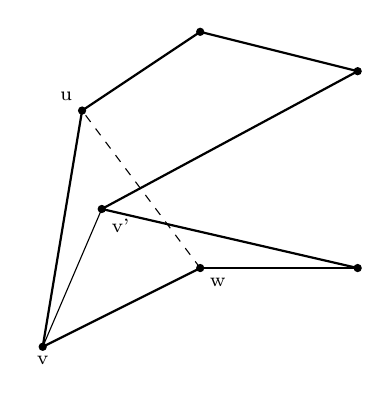
\begin{tikzpicture}[scale=1]
  % --- Define 7 vertices of a nonconvex heptagon ---
  % (Change numbers as you like)
  \coordinate (P1) at (0,0);
  \coordinate (P2) at (2,1);
  \coordinate (P3) at (4,1);
  \coordinate (P4) at (.75,1.75);
  \coordinate (P5) at (4,3.5);
  \coordinate (P6) at (2,4);
  \coordinate (P7) at (0.5,3);

  \foreach \i in {1,...,7} {
    \nextindex{\i}{7}{\next}
    \draw[thick] (P\i) -- (P\next);
    \fill (P\i) circle (1.5pt);
  }
  \node[font=\scriptsize, below] at (P1) {v};
  \node[font=\scriptsize, below right] at (P2) {w};
  \node[font=\scriptsize, above left] at (P7) {u};
  \node[font=\scriptsize, below right] at (P4) {v'};
  
  \draw[dashed]
    (P2) -- (P7);
  \draw[thin]
    (P1) -- (P4);
  
\end{tikzpicture}
\]
\caption{The two cases when trying to draw a diagonal between two points around a starting point.} \label{fig_diagonal_creation}
\end{figure}